\section{Proposed Method}
\label{sec:method}



A complete pipeline of Shape-Constrained Neural Network (SCNN) is illustrated in Figure \ref{FigSCNN}.
The framework is trained end-to-end and consists of three key components:
1) a multi-task neural network based on FCN,
2) proposed joint max pooling and
3) optimizing segmentation result with parameterized contour description.
%
\mdf{Given an input image, the first part is multi-task FCN which separately predicts a binary segmentation and shape parameter maps (Sec.~\ref{sec:multi-task-fcn}).  The two branches integrate with each other by a joint max pooling layer and contour optimization step to finally predict the shape-constrained sementation (Sec.~).}
%First, we start by introducing our multi-task neural network in Sec. \ref{Sec21}.
%And then, joint max pooling is described in detail as a tainable layer in Sec. \ref{Sec22}.
%Finally, we show how to utilize the complementary information of parameterized contour expressions to improve segmentation performance in Sec. \ref{Sec23}.



\subsection{Multi-task FCN}
\label{sec:multi-task-fcn}

\begin{figure}\label{FigMTN}
	\begin{center}
		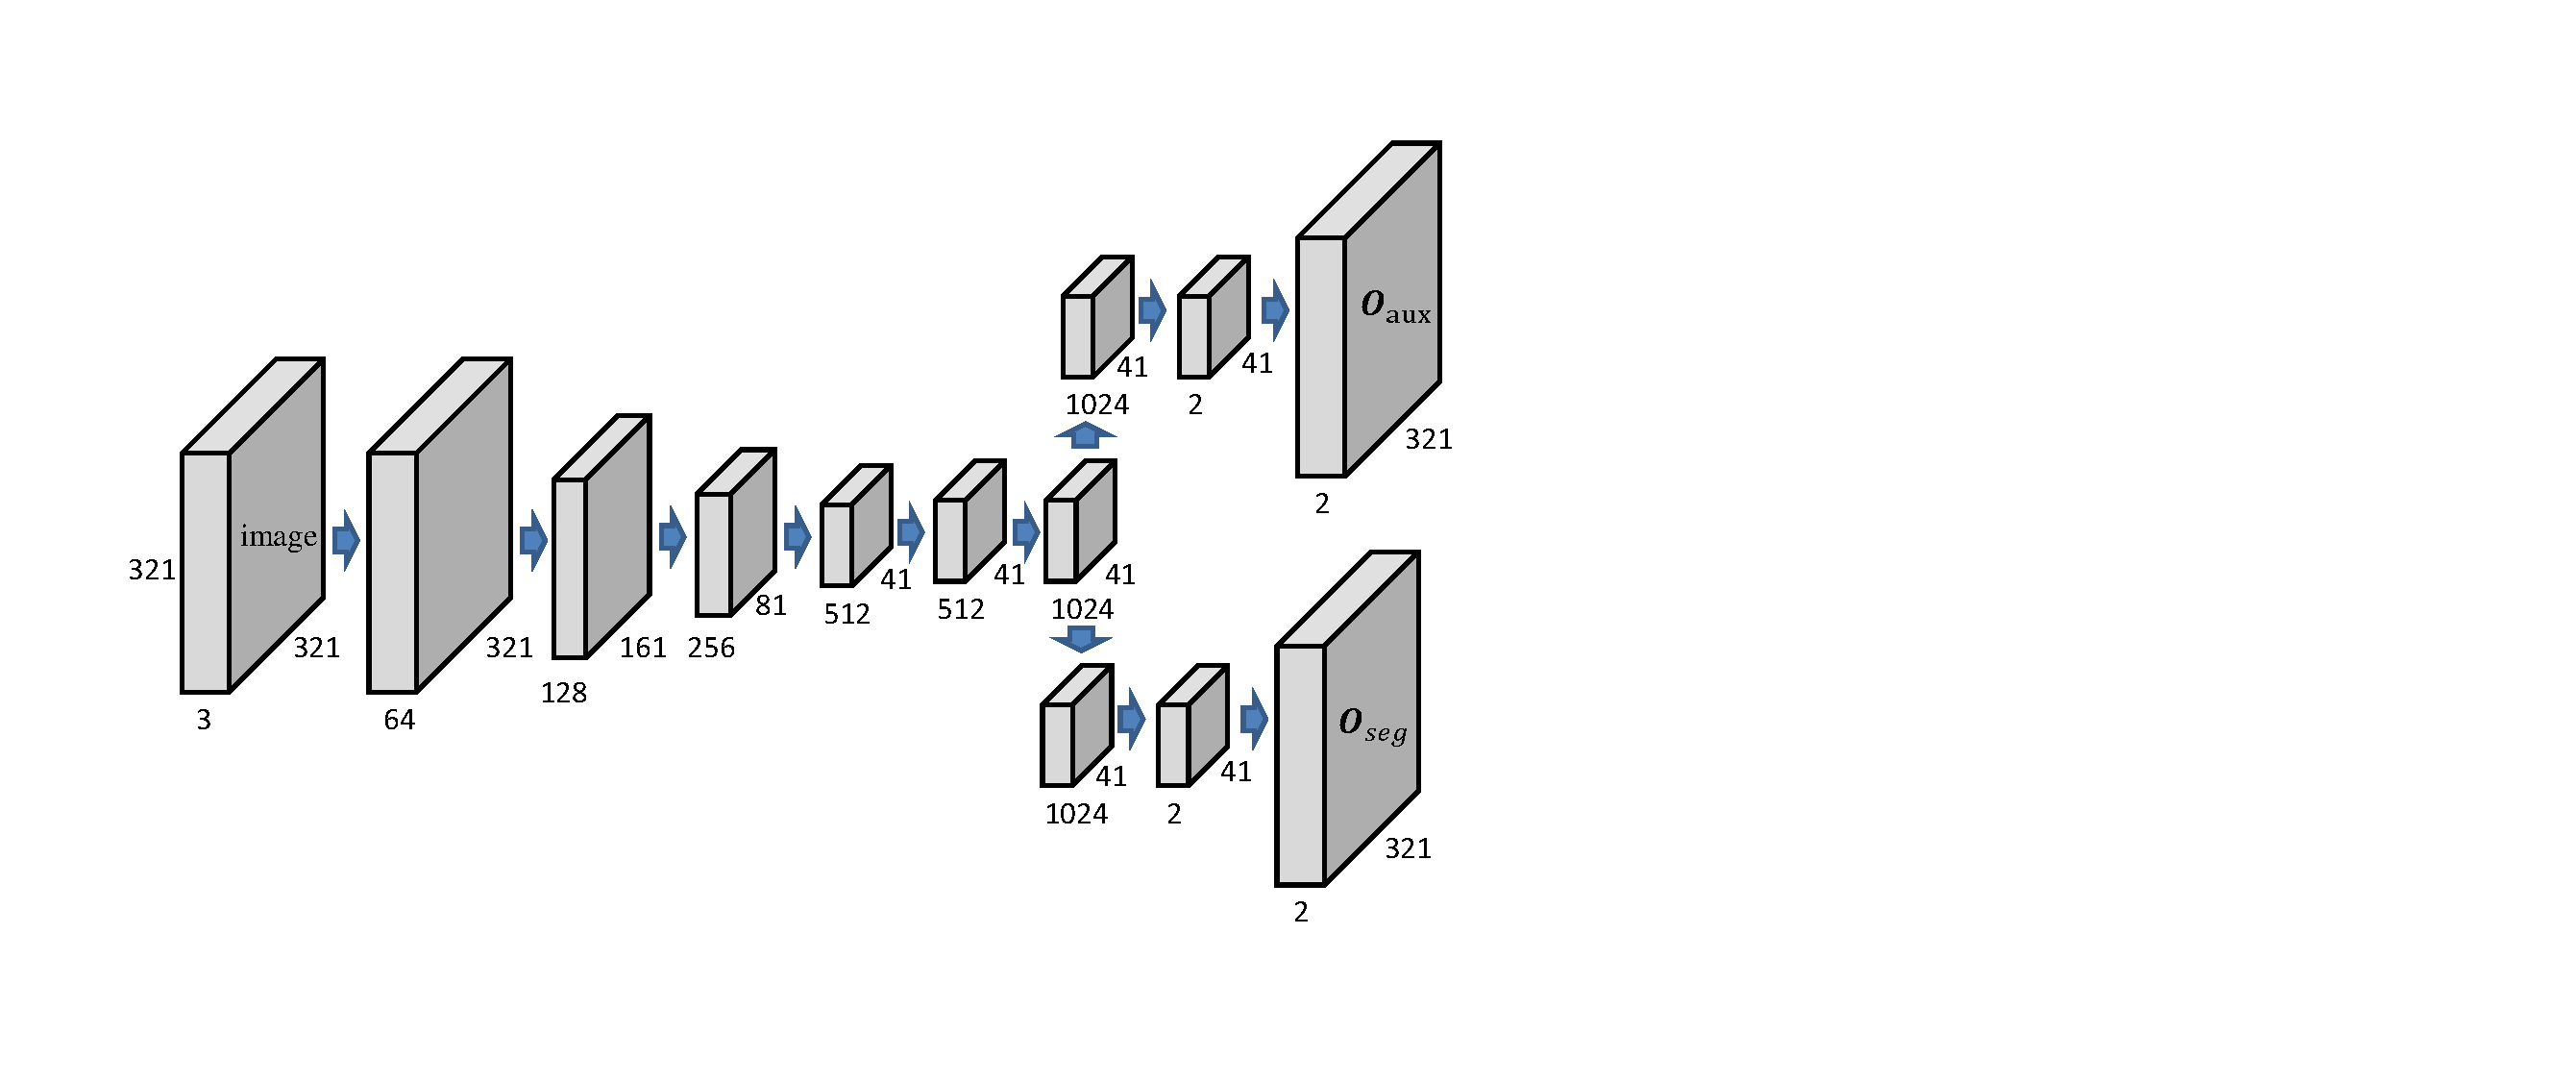
\includegraphics[width=3.3in]{figures/FigMTN.pdf}
	\end{center}
	\caption{Our multi-task network architecture. \cxj{I would sugest using real images as input and output.}}
\end{figure}

%Due to the essential ambiguity in touching regions caused by segmentation map, complementary information is needed to separate clustered objects into individuals ones.

The architecture of our multi-task learning network is shown in Figure \ref{FigMTN}.
It simultaneously predicts a segmentation map $\mathbf{M}_{seg}$ and an auxiliary map $\mathbf{M}_{aux}$ to provide complementary information.
% 
In this network, the feature learning part is shared and based on the publicly available DeepLab model~\cite{Chen2014a}, which introduces zeros into the filters to enlarge its field-Of-View \cxj{perceptive field? Why zeros in the filter can enlarge FOV?}.
%
It is initialized from VGG-16 ImageNet pretrained model.
Subsequently, feature maps output by last shared conv layer are fed into two individual branches.
In each branch, successive two conv layers, respectively with kernel size of $3\times3$ and $1\times1$, are applied to input map, and then an upsampling layer restores their resolution to the input image size.
%Especially, one branch predicts $\mathbf{O}^1_{seg}$ as a dense classification task, and the other branch predicts $\mathbf{O}^1_{aux}$ as a regression task.
During training, the parameters of shared network are jointly optimized, [copy] while the parameters of two individual branches are updated independently.

Instead of directly predicting contour probabilities like \cite{Chen2016a,Xu2016}, we choose parameterized contour description as our complementary information, which emphasizes more on the overall shape.
%
Specifically, an ellipse shape is depicted by five parameters: $\Theta = \{\theta, x_c, y_c, a, b\}$, where $\theta$ is the rotated angle of the major axis \cxj{from x-axis?}, $x_c$ and $y_c$ are the coordinates of its center, and $a$, $b$ are respectively \mdf{the lengths of the} major and minor axis.
%
Different definitions of parameters means different shape prior knowledge of object contour.
Similar to \cite{Redmon2016}, the predicted contour description on $(x,y)$ is expressed by $\mathbf{O}_{aux}(x,y) = [\theta, dx_c, dy_c, a, b]$, 
\cxj{why only on $x,y$?} 
where
\begin{eqnarray}\label{EqMax}
\begin{aligned}
\theta &= \theta^*\\
dx_c &= (x-x_c^*)/width\\
dy_c &= (y-y_c^*)/height\\
a &= a^*/width\\
b &= b^*/height\\
\end{aligned}
\end{eqnarray}
[$\theta^*$, $x_c^*$, $y_c^*$, $a^*$, $b^*$] are parameters depicting the true ellipse shape of the object to be segmented.
$width$ and $height$ are image size.
\cxj{I am confused here...}


The objective function follows the multi-task loss in Faster R-CNN~\cite{Ren2015}.
Our loss function for an image is defined as:
\begin{eqnarray}\label{EqLoss}
\begin{aligned}
L(\mathbf{O}_{seg},\mathbf{O}_{aux}) &= L_{seg}(\mathbf{O}_{seg},\mathbf{O}_{seg}^*)+\\
&\lambda L_{aux}(\mathbf{O}_{aux},\mathbf{O}_{aux}^*£¬\mathbf{O}_{seg})
\end{aligned}
\end{eqnarray}
where $L_{aux}(\mathbf{O}_{aux},\mathbf{O}_{aux}^*£¬\mathbf{O}_{seg}^*)$ only compute loss on regions with positive $\mathbf{O}_{seg}^*$ and $\lambda$ is a balancing weight.




\subsection{Joint Max Pooling}
\label{sec:joint-max-pooling}

\mdf{Based on the binary map of segmentaion and auxilary map of shape parameters obtained from the two individual branches, we now integrate these two types of information to produce more accurate boundaries.}
%
We introduce a novel joint max pooling to improve both the accuracy of segmentation and parameterized contour predictions.
Different from conventional max pooling layers, our JMP takes two inputs and pooling one with the other one.
\cxj{not clear about your key idea. You need one sentence to describe your main idea of joint pooling, how does it combine two maps..}
%JMP takes in the two outputs from previous multi-task neural networks and outputs two new predictions, as shown in Figure \ref{Fig_scnet}.

A conventional pooling operation can expressed as 
\begin{eqnarray}\label{pooling}
\begin{aligned}
y_{i,j} = \sum_{p\in \mathcal{N}_{i,j}} \omega_{p}x_{p},
\end{aligned}
\end{eqnarray}
where $\mathcal{N}_{i,j}$ a neighbor region of pixel $(i,j)$ according to the sliding window, and $\omega_{p}$ is the weight of pixel $p$.
%
For traditional max pooling, $\omega_p \in {0,1}$ is a binary indicator for that if $x_p$ is the maximum in the local region.
There is only one pixel in the neighborhood has $\omega_p=1$ and all the others have $\omega=0$.
%
For an average pooling, all pixels in the local window take the identical weight $\omega_p=\frac{1}{N}$, where $N$ is the total number of pixels in the local region $\mathcal{N}$.
%
Intuitively, $\omega$ acts like an "indictor" determining which information in $\mathbf{\overline{X}}$ should be propagated to the next layer.
Based on this observation, we proposed a split version of pooling by obtaining $\mathbf{S}$ from an independent input, instead of $\mathbf{\overline{X}}$.
%This novel split.
\begin{figure}\label{FigJMP}
\begin{center}
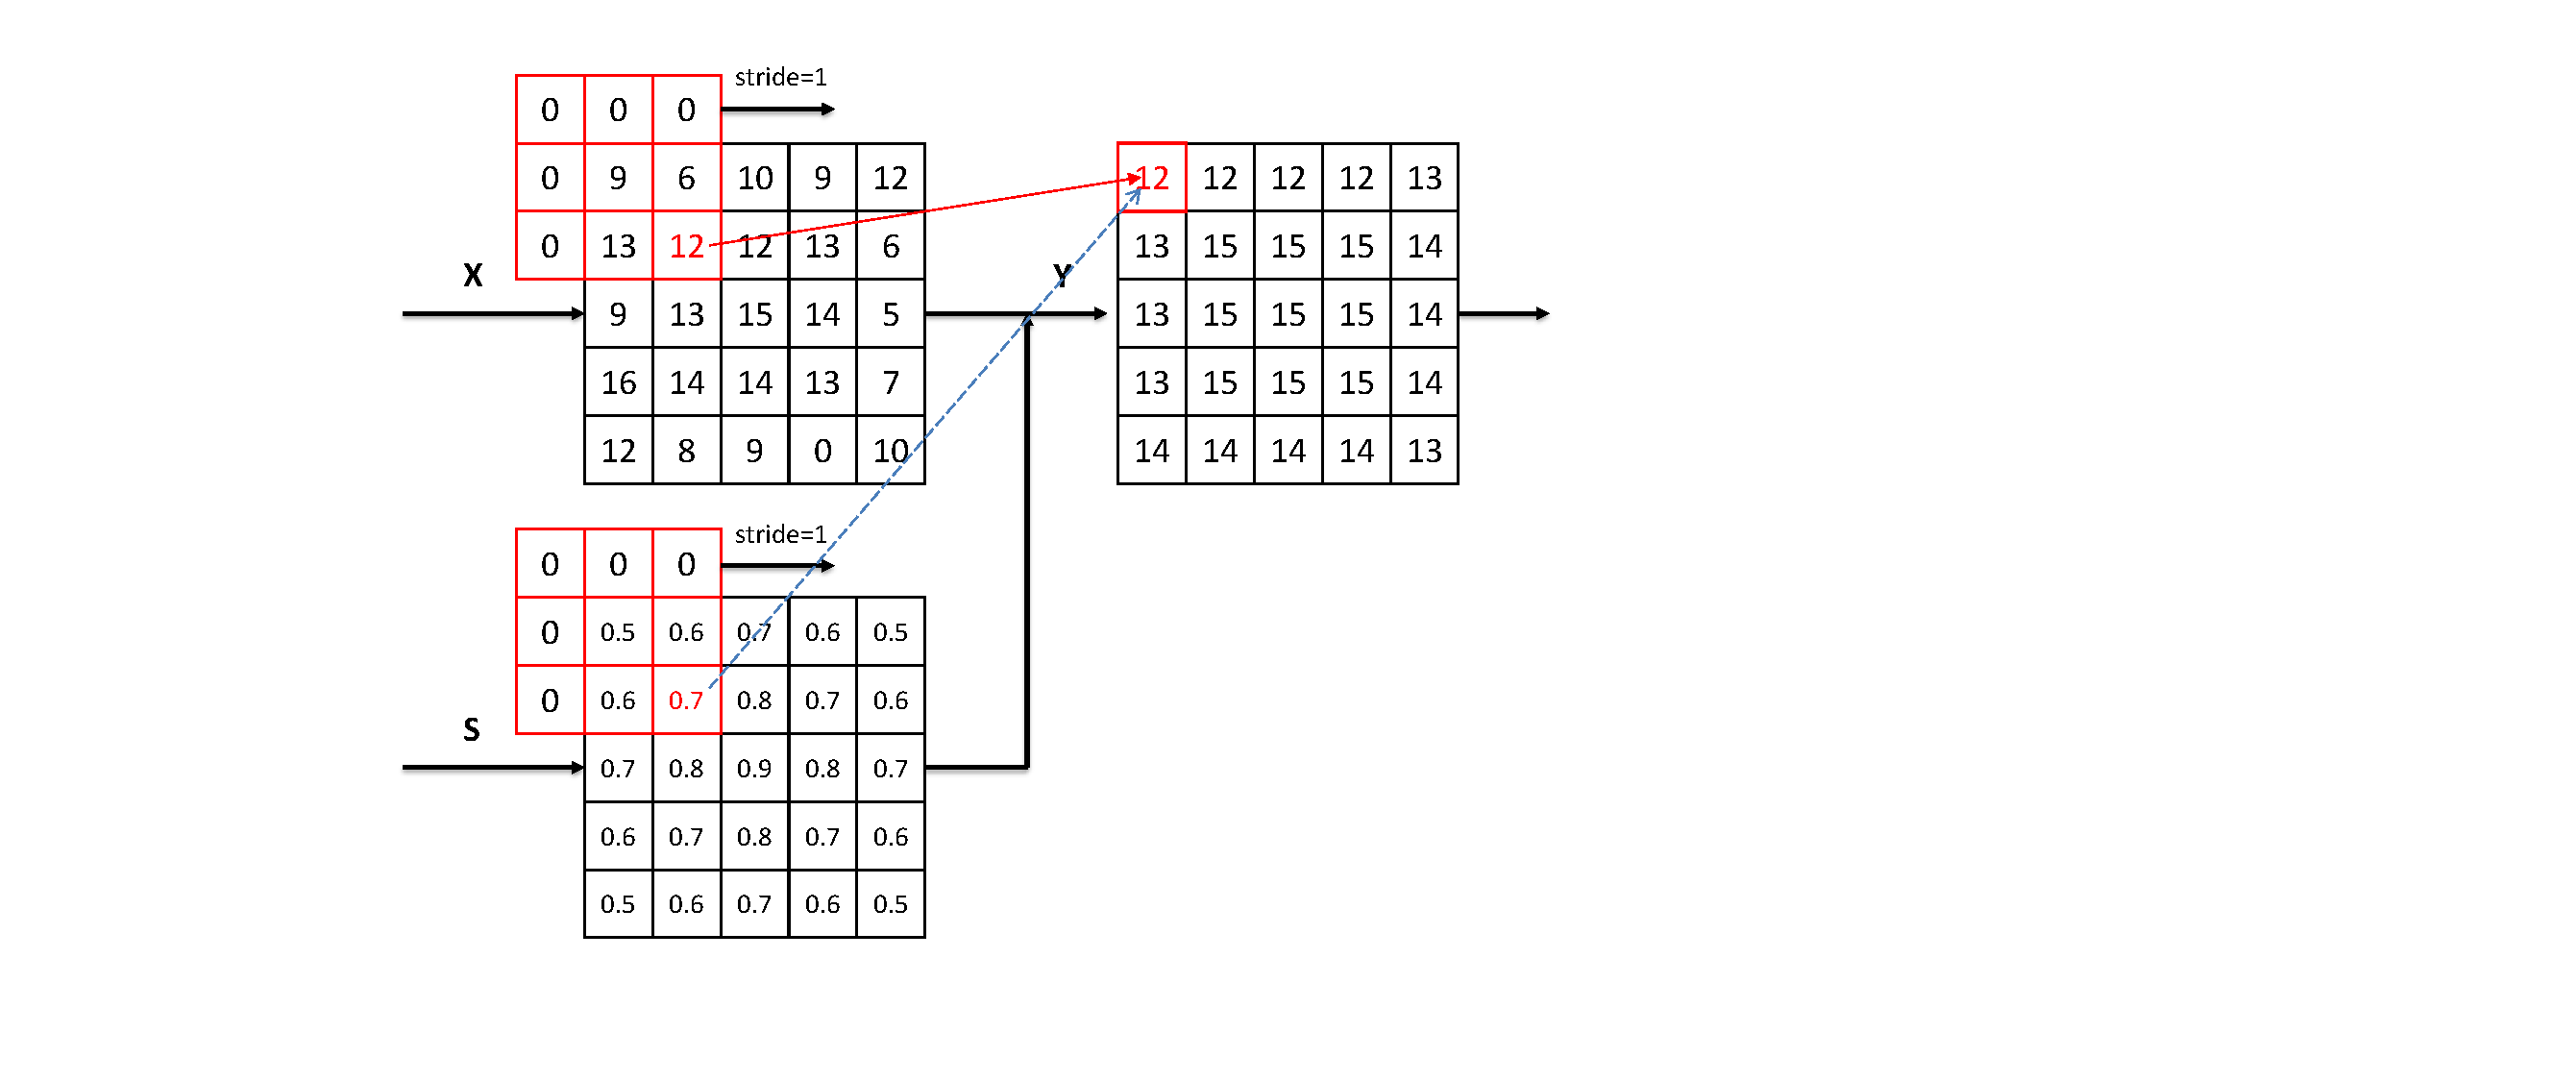
\includegraphics[width=3.4in]{figures/Fig3.pdf}
   %\includegraphics[width=0.8\linewidth]{egfigure.eps}
\end{center}
   \caption{An example of joint max pooling.
   Two windows of same size synchronously slide on $\mathbf{X}$ and $\mathbf{S}$.
   Top window will propagate the element, of which the position corresponding to bottom window has a maximum value, to next layer.
   }
\label{F3}
\end{figure}



In practice, two windows with the same size synchronously slide on two independent input.
One of the window is denoted as indicating window acting as the "indictor", while the other one is denoted as pooling windows, of which the useful information should be propagated to next layer.
In other word, elements in the indicating window determine the pooling strategy in pooling windows.
A simple example is illustrated in Figure~\ref{FigJMP}.

However for max pooling, $\mathbf{S}$ is hard to be directly learned to be binary.
Therefore we add a threshold function by:
\begin{eqnarray}\label{jmp}
\begin{aligned}
y_{\mu,\nu} &= \sum_{i,j}x_{i,j}G(s_{i,j})~~~~x_{i,j}\in \mathbf{\overline{X}},s_{i,j}\in \mathbf{S} \\
G_{\mathbf{S}}(s_{i,j},)&=\left\{\begin{array}{cc}
1&if~s_{i,j}>=max(\mathbf{S})\\
0&else\\
\end{array}\right.
\end{aligned}
\end{eqnarray}

From Figure \ref{FigJMP}, it should be noted that most elements in $\mathbf{X}$ have been substituted with the element of which the position corresponding to maximum in $\mathbf{S}$.
Therefore in our SCNN, if $\mathbf{O}_{seg}$ is denoted as $\mathbf{S}$ and $\mathbf{O}_{aux}$ is denoted as $\mathbf{X}$, only the contour description in $\mathbf{O}_{aux}$ with a local maximum objectness in $\mathbf{O}_{seg}$ can be retained by JMP.
Moreover, the discarded elements in $\mathbf{O}_{aux}$ will be replaced by a nearest retained contour description when pooling stride is set to be $1$.
%
And positions with local maximum objectness usually correspond to the center region of objects.
Especially, the kernel size and iterations of JMP determine how far a retained contour expression can be spread.
JMP guarantees the accuracy and consistency of contour description in ambiguous region of an object.

One important contribution of our JMP is that the residual error can be correctly back propagated to its inputs.
This makes it a trainable layer in any network architecture and our SCNN become a fully trainable system.
Defining $L_\mathbf{X}$ as the residual error on $\mathbf{X}$ , the back propagation for $x_{i,j}$ can be expressed by:
\begin{eqnarray}\label{bpx}
\begin{aligned}
\frac{\partial L_\mathbf{X}}{\partial x_{i,j}}=\frac{1}{m}\sum\limits_{y_{\mu,\nu}\in\mathbf{U}}\frac{\partial L_\mathbf{X}}{\partial y_{\mu,\nu}}G_{\mathbf{S}_{u,v}}(s_{i,j})\\
\end{aligned}
\end{eqnarray}
where $\mathbf{U}$ is output set $\{y_{\mu.\nu}\}$ associated with $x_{i,j}$ and $m$ is the size of $\mathbf{U}$.
${S}_{u,v}$ is the corresponding pooling window centered on ${u,v}$ of $\mathbf{X}$.
Different from conventional max pooling, Eq.~\ref{bpx} converge the gradients on the positions with local maximum $s_{i,j}$£¬ which usually are the centers of object.
%
Implementing Eq. \ref{bpx} to our SCNN can make it only focus on predicting accurate parameterized contour description on the center area of objects, instead of the whole region.


%Specially in Figure \ref{FigSCNN}, the input segmentation map is assumed to not only influence the output but also feeds a subsequent layers, thus also receiving gradient contributions $\frac{\partial L}{\partial s_{i,j}}$ from the next layer during back-propagation.

Defining $L_\mathbf{S}$ as the residual error on $\mathbf{S}$.
We assume that $s_{i,j}$ not only influences the following $y_{i,j}$ but also feeds a subsequent layer in Figure \ref{FigSCNN}, thus also receiving gradient contributions $\frac{\partial L_\mathbf{S}}{\partial s_{i,j}}$ from that layer during back-propagation.
The back propagation for $s_{i,j}$ is formulated by
%
\begin{eqnarray}\label{bps}
\begin{aligned}
\frac{\partial L_\mathbf{S}}{\partial s_{i,j}}&=\frac{\partial L_\mathbf{S}}{\partial s_{i,j}}+\frac{1}{m}\sum_{y_{\mu,\nu}\in\mathbf{U}}\frac{\partial L_\mathbf{X}}{\partial y_{\mu,\nu}}\frac{\partial y_{\mu,\nu}}{\partial s_{i,j}}\\
&=\frac{\partial L_\mathbf{S}}{\partial s_{i,j}}+\frac{1}{m}\sum_{y_{\mu,\nu}\in\mathbf{U}}\frac{\partial L_\mathbf{X}}{\partial y_{\mu,\nu}}x_{i,j}\frac{\partial G_{\mathbf{S}_{u,v}}(s_{i,j})}{\partial s_{i,j}}\\
&=\frac{\partial L_\mathbf{S}}{\partial s_{i,j}}+\sum_{y_{\mu,\nu}\in\mathbf{U}}\frac{1}{m}\frac{\partial L_\mathbf{X}}{\partial y_{\mu,\nu}}x_{i,j}\delta_{\mathbf{S}_{u,v}}(s_{i,j})\\
\end{aligned}
\end{eqnarray}
where $\delta_{\mathbf{S}_{u,v}}(s_{i,j})$ is the derived function of $G_\mathbf{S}(s_{i,j})$, which has an infinite response when $s_{i,j}=max(\mathbf{S}_{u,v})$.
In order to normally back propagate, $\frac{\partial L_\mathbf{S}}{\partial s_{i,j}}$ is approximated by:
\begin{eqnarray}\label{dG}
\begin{aligned}
\frac{\partial L_\mathbf{S}}{\partial s_{i,j}}&= \frac{\partial L_\mathbf{S}}{\partial s_{i,j}}(1+\frac{1}{m}\sum_{y_{\mu,\nu}\in\mathbf{U}}\lambda\widetilde{\delta}_{\mathbf{S}_{u,v}}(s_{i,j}))\\
\widetilde{\delta}_{\mathbf{S}_{u,v}}(s_{i,j})&=\left\{\begin{array}{cc}
1&if~s_{i,j}=max(\mathbf{S})\\
0&else\\
\end{array}\right.
\end{aligned}
\end{eqnarray}

Intuitively, Eq. \ref{dG} add\mdf{s} a loss weight on gradients of \mdf{the} local maximum $s_{i,j}$ with the control $\lambda$ (set according to iterations of JMP) to avoid false detection as much as possible.



\subsection{Fusion for Final Segmentation}
With the predicted probability maps of objectness $\mathbf{O}_{seg}$ and parameterized contour description $\mathbf{O}_{aux}$ from SCNN, the final segmentation $m(i,j)$ can be obtained by fusing them together:
%
\begin{eqnarray}\label{fusion}
\begin{aligned}
m(i,j)=\left\{\begin{array}{cc}
1&if~\mathbf{O}_{seg}(i,j)>\tau_2\\
0&if~\mathbf{O}_{seg}(i,j)<\tau_1\\
f(\mathbf{O}_{aux}(i,j))&else\\
\end{array}\right.
\end{aligned}
\end{eqnarray}
%
where $\tau_2$ and $\tau_1$ are two thresholds (set empirically) to control the degree of object contour modification by $\mathbf{O}_{aux}(i,j)$.
%
$f(\mathbf{O}_{aux}(i,j))$ is a function judging whether a position is within a shape by its coordinate $(i,j)$ and shape description $\mathbf{O}_{aux}(i,j)$.
For example in our task, we define an ellipse by $\mathbf{O}_{aux}(i,j) = [\theta, x_c, y_c, a, b]$, therefore the function is expressed by:
\begin{eqnarray}\label{fusion}
\begin{aligned}
f(\mathbf{O}_{aux}(i,j))&=\left\{\begin{array}{cc}
1&if~\frac{dx^2}{a^2}+\frac{dy^2}{b^2}<1\\
0&else\\
\end{array}\right.\\
dx &= cos(\theta)(i-x_c)+sin(\theta)(j-y_c)\\
dy &= -sin(\theta)(i-x_c)+cos(\theta)(j-y_c)\\
\end{aligned}
\end{eqnarray}

Our fusion strategy can appropriately utilize prior shape knowledge to optimize segmented object.
It can not only separate objects into individual ones, but also optimize most regular object without losing generalization to deformable objects.
The SCNN can be easily extended to other shape constraint, \mdf{such as rectangle shape, circles}, if the shape can be parameterized.
